\subsection{External interface requirements}
\subsubsection{User interfaces}

\subsubsection{Hardware interfaces}
The hardware part is mainly for both heart rate and blood oxygen saturation levels data acquisition. It also plays a part in forwarding data to an Android phone by having an NFC tag. The software part, on the other hand, is responsible for data receiving and data processing. The software application running on an Android device aims at receiving, storing and utilizing the data. After data is written to the NFC tag, an Android phone will read the tag when it is close in range. Then the measurement process in the application will start and continuously obtain data from the NFC smartwatch or from the NFC tag inside the smartphone. Indeed this hardware structure can be implemented on a smartwatch / smartring or directly on the smartphone, but in this case the data acquisition will not be continues.
\begin{figure}[h!]
  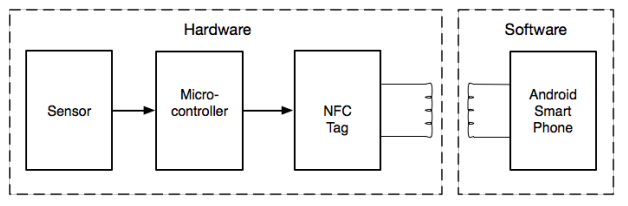
\includegraphics[width=\linewidth]{Images/hardware}
  \caption{The System Architecture.}
  \label{fig:The System Architecture}
\end{figure} 
The device must have also a GPS system for providing the position, a monitor for allowing, during the race, with the additional feature Track4Run, to see the athletes on the path, and finally the device must be able to call the 118 number.  